\section{User-facing Services}

\subsection{Portal Aspect\label{sec:portal}}

\begin{figure}
	\centering
	\scalebox{0.4}{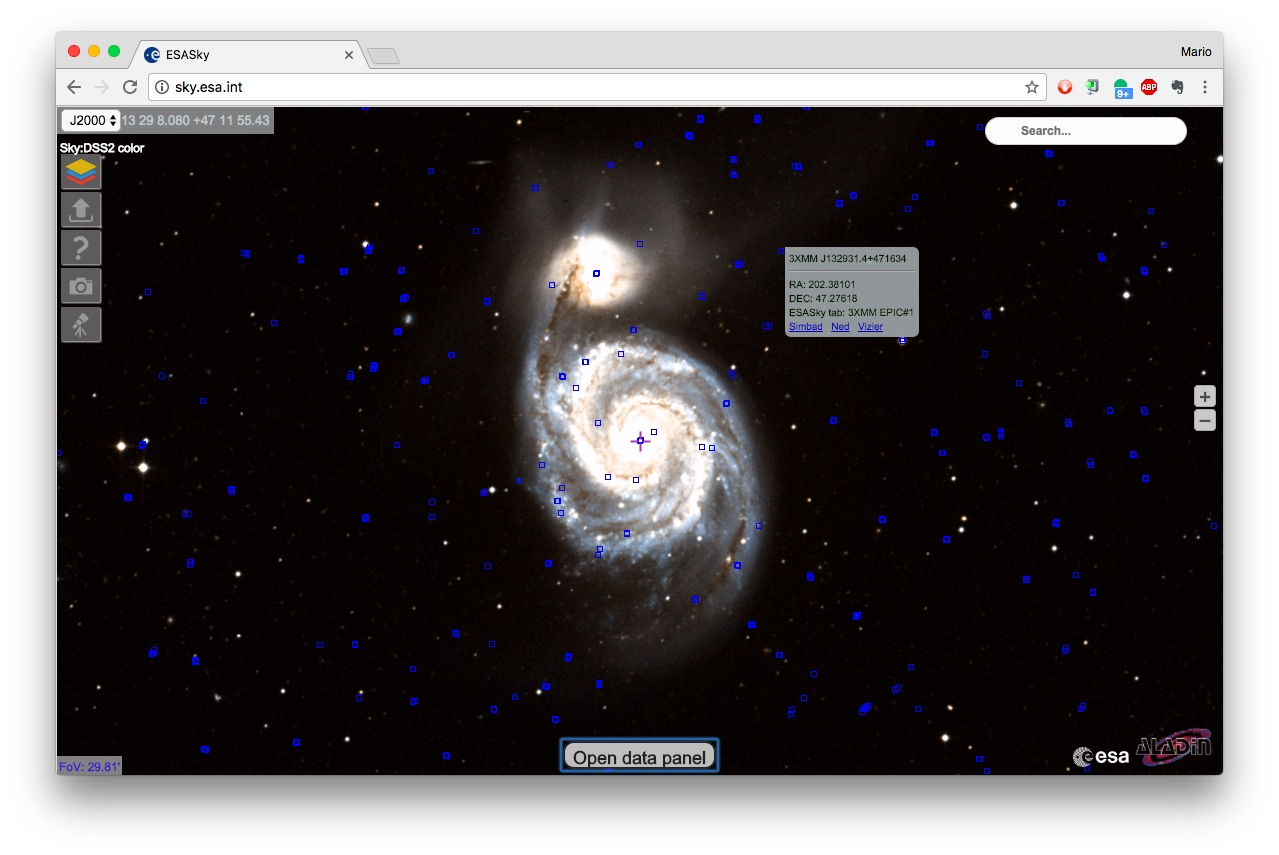
\includegraphics{images/fig-portal-esasky}}
	\caption{The "ESA Sky" web portal interface to ESA Archive holdings. The LSST portal user
		experience will support similar modern pan/zoom/select metaphor for exploration and visualization of the LSST data set.
		\label{fig:portalESA}}
\end{figure}

\begin{figure}
	\centering
	\scalebox{0.4}{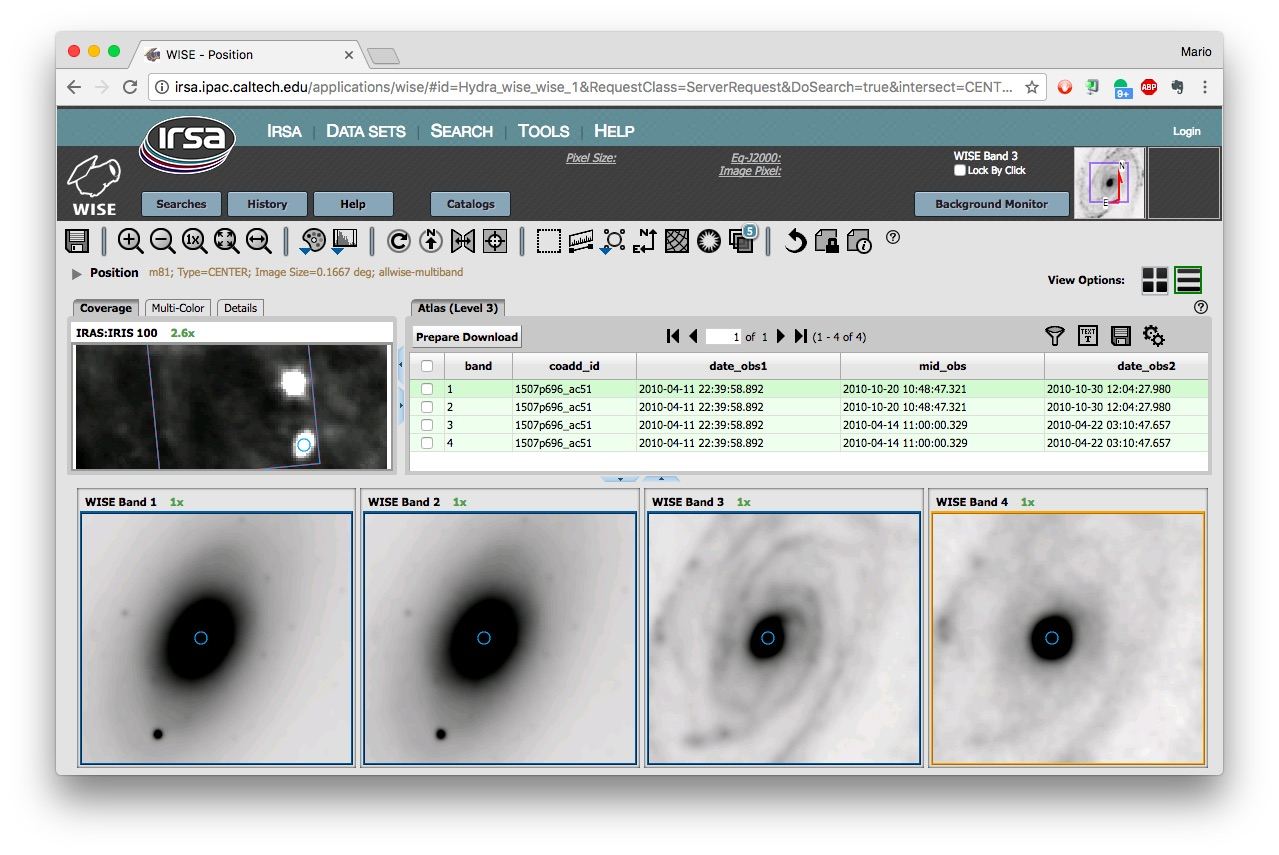
\includegraphics{images/fig-portal-irsa}}
	\caption{The web portal interface to the WISE data set at the Infra-Red Science Archive at IPAC. The LSST portal is being built by extending the Firefly toolkit that powers the IRSA/WISE archive.
		\label{fig:portalIRSA}}
\end{figure}

The \textbf{Portal Aspect} is a web portal designed to provide the essential data
access and visualization services through a simple-to-use website.  It is to
enable browsing and visualization of the available datasets in ways the
users are accustomed to at archives such as IRSA, MAST, or the SDSS archive.
To those we will add an enhanced level of interactivity in line with expectations for
then-contemporary archive portals (similar to that found today in ESASky and
the DECaLS Viewer). Examples of the types of user experiences to be offered
through the LSST portal are shown in Figures~\ref{fig:portalESA}~and~\ref{fig:portalIRSA}.

Through the Portal, the users will be
able to view the LSST images, request subsets of data (via simple forms or
ADQL queries), store the results of such queries to their personal
workspaces, as well as download them. The Portal will also make it possible to
construct commonly requested plots, and generally explore the
LSST dataset in a way that allows the users to identify and access (subsets of)
data required by their science case.

Virtually all LSST users will use the Portal as their first point of entry to
access and explore the LSST data set. When developing the Portal,
we will therefore \textbf{emphasize the user experience and exploratory
capabilities}, over analysis features. The latter are expected to be more
directly satisfied by the Notebook Aspect.

\subsection{Notebook (JupyterLab) Aspect\label{sec:jupyter}}

\begin{figure}
	\centering
	\scalebox{0.6}{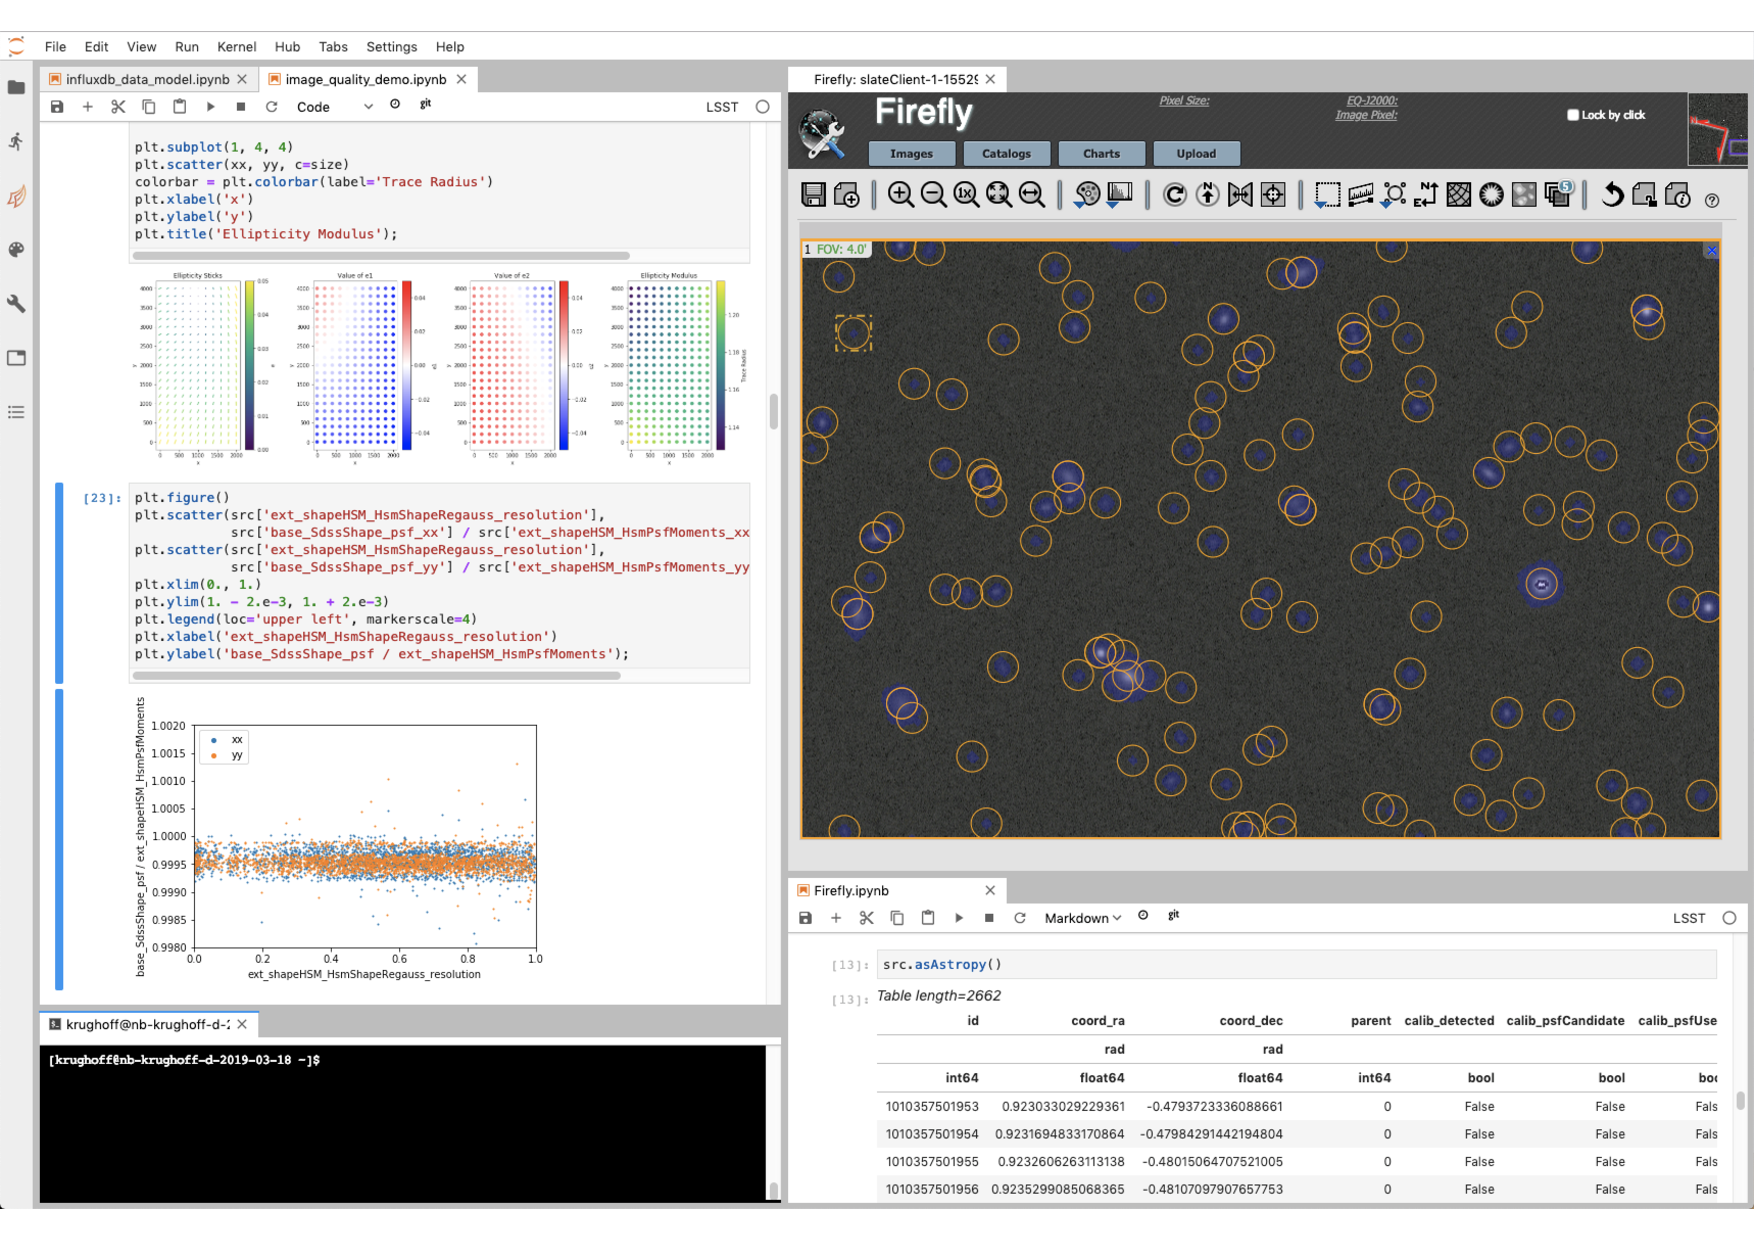
\includegraphics[scale=0.9]{images/fig-notebook-imagequality}}
	\caption{A screen capture of the Notebook interface running LSST image processing code within a notebook. \label{fig:JupyterLab}}
\end{figure}

The \textbf{Notebook Aspect}
%, based on the Jupyter family of technologies (such as JupyterHub and JupyterLab),
will be provided to allow for more sophisticated data selection, analysis, and creation of added value \emph{User Generated} data products.
A screen capture of a mature prototype of the Notebook Aspect is shown in Figure~\ref{fig:JupyterLab}.

The Notebook Aspect user experience will be nearly identical to working with
Jupyter notebooks locally, except that computation and analysis will occur
at resources provided at the LSST Data Access Center.
This is an
implementation of the ``bringing analysis to the data'' paradigm: rather
than imposing the burden of downloading, storing, and processing (large)
subsets of LSST data at their home institutions, we will enable our users to
bring their codes to and perform their analysis at the LSST DAC.  We expect
this will reduce the barrier to entry and shorten the path to science for
the LSST science community.

We will provide JupyterLab instances to LSST users in an environment carrying a
library of preinstalled commonly used and useful software tools:
Astropy, the LSST science pipelines, Anaconda Scientific Python Distribution, the PyViz visualization toolkit, and others.
The users will be able to upload and install their own tools as well.
Non-trivial shared computing cluster resources will be accessible through this environment as well, enabling the generation of \emph{User Generated} data products.

% Add something about writing glue code to make it easy to submit jobs, and how Notebooks will be the primary user interface to the backend batch system...

The Notebook Aspect of the science platform will play a key role in commissioning,
quality assessment, and science validation of the as-built system.
It will be the primary method of performing interactive analysis of acquired data
(e.g., adjusting and executing prepared notebooks driving commissioning tasks).
Through the terminal functionality of the JupyterLab environment, it will also permit commanding the batch resources to execute larger processing tasks.
Due to this, we expect the
Notebook Aspect to reach maturity earlier than the others, and certainly in time for
commissioning.

% Data sets acquired during commissioning, as well as precursor and simulated data sets processed for quality assessment and science validation while construction is ongoing, will appear in the commissioning workspace, ready for operator analysis using tools and

\subsection{Web API Aspect\label{sec:apis}}

\begin{figure}
	\centering
	\scalebox{0.4}{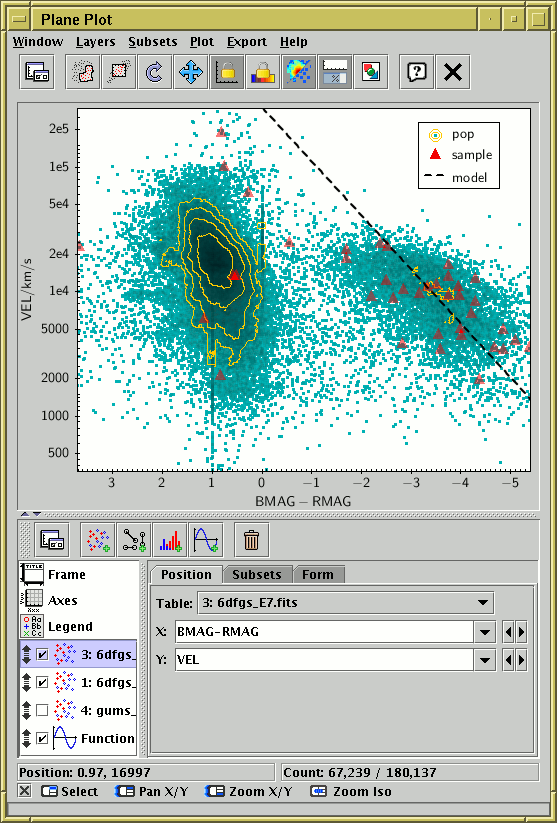
\includegraphics[scale=0.7]{images/topcat-StackPlotWindow}}
	\caption{A screen capture of Tool for OPerations on Catalogues And Tables (TOPCAT), that is capable of remotely accessing catalogs using VO protocols. Tools such as these will be able to directly access the data sets served by the LSST DACs (figure credit: Mark Taylor, \url{http://www.star.bris.ac.uk/~mbt/topcat/sun253/sun253.html}).
		\label{fig:toolsTOPCAT}}
\end{figure}

Backend Platform services --- such as access to
databases, images, and other files --- will be exposed to the public Internet through
machine-accessible web APIs.
These will serve the data using community-accepted
formats and protocols, making it easy to remotely access the LSST data and DAC	
services.
Furthermore, to ensure maximal exposure of the DAC services through the Web APIs,
the other two Aspects of the Platform --- Portal and Notebook --- will
internally access the LSST datasets using the same Web APIs to the greatest extent possible.

Exposing the LSST data through Virtual Observatory interfaces plays a particularly important role.
This will allow the discoverability of LSST data products from within the Virtual Observatory,
and federation of the LSST data set to other archives.
It will also enable the use of widely utilized tools such as TOPCAT or DS9 by the end-users,
further lowering the barrier to access to LSST data, and shortening the path to science.
It will also allow these tools to be used in commissioning,
easing the way for scientists new to the LSST environment to access the data and make meaningful
contributions to this time-compressed activity.

LSST will follow a ``VO-first'' strategy, using IVOA-standard interfaces wherever practical,
though we may also provide some services using custom protocols in areas where relevant standards have not yet been developed.
LSST will actively participate in the IVOA community, and will propose evolutions of standards when we find problems and where we feel that our custom work could be of broader benefit to the community.
We will also use our engagement with the IVOA to ensure that we are following mainstream interpretations of the standards and to maintain contact with the authors of client software such as TOPCAT.

Additional details on the standards to be supported are provided below.

\subsection{Integrated environment}

All the Aspects of the LSST Science Platform are intended to be \emph{well integrated}, enabling a seamless workflow so the users will be able to move back and forth between them as needs dictate.
The aim is to enable a user to find or create data in one Platform Aspect, and view or analyze that data in another.

As an example of how these connections can aid a user in exploring the LSST data, data queries will be shareable across the Portal, Notebook, and Web API Aspects.
This will allow a user to build a query using the Portal's TAP query UI component, view the (possibly preliminary) results by browsing them in place in the Portal, and then access the final results from a JupyterLab notebook or a remotely connected client (e.g., TOPCAT) for further analysis.
The reverse flow will also be enabled; a user can code and submit a complex SQL query in the Notebook, and then browse and visualize the results in the Portal.

By making the environments integrated, we allow for a shallower learning curve and a gradual transition to more complex environments at the point they are needed.
For example, a user may begin interacting with the LSST dataset using the Portal Aspect but may ultimately reach the limitations of the selection and analysis tools it provides.
The integrated nature of the platform will allow such a user to switch to the Notebook Aspect, and continue working on the data analysis started in the Portal.
There, they will be able to import the analysis artifacts (e.g., catalog subsets) as standard Python objects (e.g., as astropy.table).

\subsection{Next to Data Processing\label{sec:n2d}}
Many LSST science cases will require analysis of the full LSST Object and/or Source tables; subsetting and downloading reduced catalogs will not suffice for science that requires, for example, fitting and computing features of light curves for large numbers of Objects, creating maps of stellar density, or training machine learning models.
The LSST Object table alone will be $\approx$~50TB for Data Release 1 and $\approx$~300TB for Data Release 11 at the close of the 10-year survey.
The LSST Science Platform will enable user-driven large-scale search and analysis capabilities of the LSST data by providing a \emph{Next-to-Data} processing environment, allowing users to bring their analysis to the data.
This environment will be supported by backend services, as described in \ref{sec:backend}

\subsection{Supporting Collaborative Work\label{sec:collab}}

The LSST Science Platform will provide support for collaborative work at two levels:
\begin{itemize}
	\item \textbf{Shared workspaces}: Creation and sharing of data sets --- catalogs, images, queries, and other data products --- within either pre-defined or dynamically-created groups (e.g., a research group at a university, or a large science collaboration).
Such groups would have access to a shared virtual ``workspace'' within the LSST DAC.
This workspace will include shared files, shared catalogs (stored in user databases) as well as computing cycles allocated to the group as a whole.
This shared workspace will be equally ``visible'' from all three Aspects of the platform --- e.g., uploads to the workspace will be possible either through a form in the Portal, POSIX-style file access from JupyterLab, or using an external file transfer client via WebDAV or VOSpace.

	\item \textbf{Shared editing}: Although we have no formal requirement to provide shared editing capabilities, we envisage supporting ``Google Docs''-like collaborative editing, visualization, and data analysis capabilities, via the integration of 3rd-party tools, \emph{if and when these technologies become available in upstream products}.
	% At present, collaborative editing is on the development roadmap for Jupyter Notebooks, and will be included into our Notebook Aspect as it reaches production quality.
\end{itemize}

The levels of support for collaboration described above are responsive to the large majority of user needs identified by end-user focus groups in R\&D. At the same time, they minimize the technical risks by leveraging widely used and well understood technologies (SDSS-like MyDB user databases, backend authentication \& authorization mechanisms, VO protocols, Jupyter).
